\documentclass[12pt,a4paper]{article}
\usepackage{amsmath, amssymb, geometry, booktabs, xcolor, hyperref,
            listings, pgfplots, tcolorbox, enumitem, fancyhdr, tikz, array}
\usepgfplotslibrary{fillbetween}
\geometry{margin=2.5cm}
\pgfplotsset{compat=1.18}
\tcbuselibrary{skins, breakable}

% Define custom environments
\newtcolorbox{curiositybox}[1]{colback=yellow!10, colframe=orange!80, title=#1, breakable}
\newtcolorbox{infobox}[1]{colback=blue!5, colframe=blue!60, title=#1, breakable}
\newtcolorbox{mistakebox}[1]{colback=red!5, colframe=red!60, title=#1, breakable}
\newtcolorbox{learnbox}[1]{colback=green!5, colframe=green!60, title=#1, breakable}

% Header and Footer
\pagestyle{fancy}
\fancyhf{}
\lhead{Cayley-Hamilton Theorem}
\rhead{Unit 2 -- LAC}
\cfoot{\thepage}

% Document Title Setup
\title{\textbf{Cayley-Hamilton Theorem} \\ \large Unit 2 -- Eigenvalues, Eigenvectors, Diagonalization and Quadratic Forms}
\author{Department of Mathematics}
\date{\today}

\begin{document}
\maketitle
\tableofcontents
\newpage

%=============================================================
\section{Real-World Engineering Hook}
%=============================================================

\begin{curiositybox}{Why Should an Engineer Care?}
Imagine you are designing a discrete-time control system for a robot arm.
The state of the system at step $k$ is given by $\mathbf{x}_{k} = A^{k}\mathbf{x}_{0}$,
where $A$ is a $4\times 4$ state matrix.
To predict the arm's position 100 steps ahead, you naively need $A^{100}$---a
daunting computation.

The \textbf{Cayley-Hamilton Theorem} rescues you: because $A$ satisfies its own
characteristic polynomial $p(\lambda) = 0$, the equation $p(A) = \mathbf{0}$
lets you \emph{reduce} any power $A^{n}$ (no matter how large) to a polynomial
in $A$ of degree at most $3$ (one less than the matrix size).
Suddenly, computing $A^{100}$ costs the same as computing $A^{3}$.

The same trick appears in:
\begin{itemize}
  \item \textbf{State-space control:} computing matrix exponentials $e^{At}$ for
        continuous-time systems.
  \item \textbf{Digital signal processing:} evaluating IIR filter response matrices
        without brute-force multiplication.
  \item \textbf{Structural dynamics:} finding the inverse of a stiffness matrix
        without Gaussian elimination, using only matrix multiplications.
\end{itemize}
The Cayley-Hamilton Theorem is the algebraic Swiss Army knife of applied linear
algebra---and after this lecture, you will wield it fluently.
\end{curiositybox}

%=============================================================
\section{Why This Topic Exists}
%=============================================================

\begin{center}
\begin{tabular}{@{}p{3.8cm} p{5.2cm} p{6cm}@{}}
\toprule
\textbf{Atomic Sub-Topic} & \textbf{Core Mathematical Idea} & \textbf{Engineering Consequence} \\
\midrule
Statement \& Proof Sketch &
Every square matrix $A$ satisfies $p(A)=\mathbf{0}$ where $p$ is its characteristic polynomial &
Guarantees algebraic identities exist for \emph{every} square system matrix, enabling symbolic reduction \\
\addlinespace
Verification (2\(\times\)2 \& 3\(\times\)3) &
Direct substitution: compute $p(A)$ term by term and confirm the zero matrix &
Provides engineers a sanity-check routine before applying CH-based algorithms in code \\
\addlinespace
Finding Inverse via CH &
Isolate $A^{-1}$ from $p(A)=\mathbf{0}$ as a polynomial in $A$ &
Avoids row-reduction for matrix inversion; critical in real-time embedded control where Gaussian elimination is costly \\
\addlinespace
Computing Powers via CH &
Reduce $A^{n}$ to a polynomial of degree $\leq n-1$ by repeated use of $p(A)=\mathbf{0}$ &
Enables efficient long-horizon state prediction and matrix exponential approximation in simulation \\
\addlinespace
Minimal Polynomial &
Lowest-degree monic polynomial annihilating $A$; divides the characteristic polynomial &
Determines the exact degree of polynomial needed for reduction---smaller degree means faster algorithms \\
\bottomrule
\end{tabular}
\end{center}

\begin{learnbox}{Learning Objectives}
After studying this topic you will be able to:
\begin{enumerate}
  \item State the Cayley-Hamilton Theorem precisely and outline its proof for $2\times 2$ matrices.
  \item Verify the theorem by direct substitution for $2\times 2$ and $3\times 3$ matrices.
  \item Compute the inverse $A^{-1}$ of an invertible matrix using the CH relation.
  \item Reduce high matrix powers $A^{n}$ to low-degree polynomials in $A$.
  \item Define the minimal polynomial, relate it to the characteristic polynomial, and identify cases where they differ.
\end{enumerate}
\end{learnbox}

%=============================================================
\section{Intuition First and Mathematical Definitions}
%=============================================================

%---------------------------------------------------------
\subsection{Statement and Proof Sketch}
%---------------------------------------------------------

Think of the characteristic polynomial $p(\lambda) = \det(\lambda I - A)$ as a
``description'' of the matrix $A$.
Ordinarily we solve $p(\lambda) = 0$ to find scalar eigenvalues.
The Cayley-Hamilton Theorem says: \emph{plug the matrix itself in for $\lambda$},
and the result is the zero matrix.
The matrix, in a precise sense, is its own eigenvalue.

\begin{infobox}{Cayley-Hamilton Theorem --- Statement and Proof Sketch}
\textbf{Theorem (Cayley-Hamilton):}
Let $A$ be an $n\times n$ matrix over $\mathbb{R}$ (or $\mathbb{C}$) and let
\[
  p(\lambda) = \det(\lambda I - A) = \lambda^{n} + c_{n-1}\lambda^{n-1} + \cdots + c_{1}\lambda + c_{0}
\]
be its characteristic polynomial.  Then
\[
  p(A) = A^{n} + c_{n-1}A^{n-1} + \cdots + c_{1}A + c_{0}I = \mathbf{0}.
\]

\textbf{Proof Sketch for $2\times 2$:}
Let $A = \begin{pmatrix} a & b \\ c & d \end{pmatrix}$.
Then $p(\lambda) = \lambda^{2} - (a+d)\lambda + (ad-bc)$.
We need to show $p(A) = A^{2} - (a+d)A + (ad-bc)I = \mathbf{0}$.

Compute $A^{2}$:
\[
  A^{2} = \begin{pmatrix} a^{2}+bc & b(a+d) \\ c(a+d) & bc+d^{2} \end{pmatrix}.
\]
Compute $(a+d)A$:
\[
  (a+d)A = \begin{pmatrix} a(a+d) & b(a+d) \\ c(a+d) & d(a+d) \end{pmatrix}.
\]
Compute $(ad-bc)I$:
\[
  (ad-bc)I = \begin{pmatrix} ad-bc & 0 \\ 0 & ad-bc \end{pmatrix}.
\]
Subtracting:
\[
  p(A) = A^{2} - (a+d)A + (ad-bc)I
       = \begin{pmatrix} a^{2}+bc - a(a+d) + ad-bc & 0 \\ 0 & bc+d^{2}-d(a+d)+ad-bc \end{pmatrix}
       = \begin{pmatrix} 0 & 0 \\ 0 & 0 \end{pmatrix} = \mathbf{0}. \quad \checkmark
\]

\textbf{Key consequence:} $p(A) = \mathbf{0}$ is an algebraic identity that holds
for \emph{every} square matrix, regardless of whether it is diagonalisable.
\end{infobox}

\textbf{Worked Example 3.1 --- Verifying the theorem statement for a specific $2\times 2$ matrix:}

Let $A = \begin{pmatrix} 3 & 1 \\ 2 & 4 \end{pmatrix}$.

Step 1: Characteristic polynomial.
\[
  p(\lambda) = \det\!\begin{pmatrix} \lambda-3 & -1 \\ -2 & \lambda-4 \end{pmatrix}
             = (\lambda-3)(\lambda-4) - (-1)(-2)
             = \lambda^{2} - 7\lambda + 10.
\]

Step 2: By CH, $p(A) = A^{2} - 7A + 10I$ should equal $\mathbf{0}$.

Step 3: Compute $A^{2}$.
\[
  A^{2} = \begin{pmatrix} 3 & 1 \\ 2 & 4 \end{pmatrix}\begin{pmatrix} 3 & 1 \\ 2 & 4 \end{pmatrix}
        = \begin{pmatrix} 9+2 & 3+4 \\ 6+8 & 2+16 \end{pmatrix}
        = \begin{pmatrix} 11 & 7 \\ 14 & 18 \end{pmatrix}.
\]

Step 4: Compute $7A$.
\[
  7A = \begin{pmatrix} 21 & 7 \\ 14 & 28 \end{pmatrix}.
\]

Step 5: Compute $10I$.
\[
  10I = \begin{pmatrix} 10 & 0 \\ 0 & 10 \end{pmatrix}.
\]

Step 6: $p(A) = A^{2} - 7A + 10I$.
\[
  p(A) = \begin{pmatrix} 11 & 7 \\ 14 & 18 \end{pmatrix}
       - \begin{pmatrix} 21 & 7 \\ 14 & 28 \end{pmatrix}
       + \begin{pmatrix} 10 & 0 \\ 0 & 10 \end{pmatrix}
       = \begin{pmatrix} 0 & 0 \\ 0 & 0 \end{pmatrix} = \mathbf{0}. \quad \checkmark
\]
The theorem is confirmed.

%---------------------------------------------------------
\subsection{Verification for $2\times2$ and $3\times3$ Matrices}
%---------------------------------------------------------

The best way to build confidence in any theorem is to verify it with your own
hands on specific numbers.
For a $2\times 2$ matrix, you substitute $A$ into a degree-2 polynomial and check
four entries go to zero.
For a $3\times 3$ matrix, the polynomial is degree 3 and you check nine entries---it
is more arithmetic, but the logic is identical.

\begin{infobox}{Verification Procedure}
\textbf{Algorithm for verification:}
\begin{enumerate}
  \item Compute $p(\lambda) = \det(\lambda I - A)$.
        \begin{itemize}
          \item $2\times2$: $p(\lambda) = \lambda^{2} - \operatorname{tr}(A)\,\lambda + \det(A)$.
          \item $3\times3$: $p(\lambda) = \lambda^{3} - \operatorname{tr}(A)\,\lambda^{2}
                 + \tfrac{1}{2}[(\operatorname{tr}A)^{2}-\operatorname{tr}(A^{2})]\,\lambda - \det(A)$.
        \end{itemize}
  \item Form $p(A)$ by replacing $\lambda^{k}$ with $A^{k}$ and $\lambda^{0}$ with $I$.
  \item Compute $A^{2}$ and $A^{3}$ (if needed) by matrix multiplication.
  \item Substitute and confirm every entry is zero.
\end{enumerate}

\textbf{Useful identities for $2\times2$:}
\[
  p(\lambda) = \lambda^{2} - \operatorname{tr}(A)\,\lambda + \det(A), \qquad
  p(A) = A^{2} - \operatorname{tr}(A)\,A + \det(A)\,I = \mathbf{0}.
\]
\end{infobox}

\textbf{Worked Example 3.2 --- Verification for a $3\times3$ matrix:}

Let $B = \begin{pmatrix} 1 & 0 & 2 \\ 0 & 2 & 1 \\ 1 & 0 & 3 \end{pmatrix}$.

Step 1: $\operatorname{tr}(B) = 1+2+3 = 6$.

Step 2: $\det(B)$. Expanding along the first row:
\begin{align*}
  \det(B) &= 1\cdot\det\begin{pmatrix}2&1\\0&3\end{pmatrix}
             - 0 + 2\cdot\det\begin{pmatrix}0&2\\1&0\end{pmatrix} \\
          &= 1\cdot(6-0) + 2\cdot(0-2) = 6 - 4 = 2.
\end{align*}

Step 3: Second symmetric function
$s_{2} = \tfrac{1}{2}[(\operatorname{tr}B)^{2}-\operatorname{tr}(B^{2})]$.

Compute $B^{2}$:
\[
  B^{2} = \begin{pmatrix} 1&0&2\\0&2&1\\1&0&3 \end{pmatrix}
          \begin{pmatrix} 1&0&2\\0&2&1\\1&0&3 \end{pmatrix}
        = \begin{pmatrix} 1+0+2 & 0+0+0 & 2+0+6 \\
                          0+0+1 & 0+4+0 & 0+2+3 \\
                          1+0+3 & 0+0+0 & 2+0+9 \end{pmatrix}
        = \begin{pmatrix} 3&0&8\\1&4&5\\4&0&11 \end{pmatrix}.
\]
$\operatorname{tr}(B^{2}) = 3+4+11 = 18$.
$s_{2} = \tfrac{1}{2}(36 - 18) = 9$.

Step 4: Characteristic polynomial:
\[
  p(\lambda) = \lambda^{3} - 6\lambda^{2} + 9\lambda - 2.
\]

Step 5: Form $p(B) = B^{3} - 6B^{2} + 9B - 2I$.

Compute $B^{3} = B^{2}\cdot B$:
\[
  B^{3} = \begin{pmatrix}3&0&8\\1&4&5\\4&0&11\end{pmatrix}
          \begin{pmatrix}1&0&2\\0&2&1\\1&0&3\end{pmatrix}
        = \begin{pmatrix}3+0+8&0+0+0&6+0+24\\1+0+5&0+8+0&2+4+15\\4+0+11&0+0+0&8+0+33\end{pmatrix}
        = \begin{pmatrix}11&0&30\\6&8&21\\15&0&41\end{pmatrix}.
\]

Step 6: Compute each term.
\[
  6B^{2} = \begin{pmatrix}18&0&48\\6&24&30\\24&0&66\end{pmatrix}, \quad
  9B = \begin{pmatrix}9&0&18\\0&18&9\\9&0&27\end{pmatrix}, \quad
  2I = \begin{pmatrix}2&0&0\\0&2&0\\0&0&2\end{pmatrix}.
\]

Step 7: $p(B) = B^{3} - 6B^{2} + 9B - 2I$:
\[
  p(B) = \begin{pmatrix}11-18+9-2&0&30-48+18-0\\6-6+0-0&8-24+18-2&21-30+9-0\\15-24+9-0&0&41-66+27-2\end{pmatrix}
        = \begin{pmatrix}0&0&0\\0&0&0\\0&0&0\end{pmatrix} = \mathbf{0}. \quad \checkmark
\]

%---------------------------------------------------------
\subsection{Finding the Inverse Using CH}
%---------------------------------------------------------

The CH relation $p(A) = \mathbf{0}$ is a polynomial equation in $A$.
If $A$ is invertible then $c_{0} = \det(A) \neq 0$, so we can solve the
constant term for $I$, then multiply by $A^{-1}$ to get a neat formula for
the inverse using only powers of $A$---no row operations needed.

\begin{infobox}{Inverse via the Cayley-Hamilton Theorem}
Let $A$ be an $n\times n$ \emph{invertible} matrix with characteristic polynomial
\[
  p(\lambda) = \lambda^{n} + c_{n-1}\lambda^{n-1} + \cdots + c_{1}\lambda + c_{0},
  \quad c_{0} = (-1)^{n}\det(A) \neq 0.
\]
From $p(A) = \mathbf{0}$:
\[
  A^{n} + c_{n-1}A^{n-1} + \cdots + c_{1}A + c_{0}I = \mathbf{0}.
\]
Multiply both sides on the left (or right) by $A^{-1}$:
\[
  A^{n-1} + c_{n-1}A^{n-2} + \cdots + c_{1}I + c_{0}A^{-1} = \mathbf{0}.
\]
Isolate $A^{-1}$:
\[
  \boxed{A^{-1} = -\frac{1}{c_{0}}\!\left(A^{n-1} + c_{n-1}A^{n-2} + \cdots + c_{1}I\right).}
\]

\textbf{For $2\times2$:}
$p(\lambda) = \lambda^{2} - \operatorname{tr}(A)\lambda + \det(A)$,
so $c_{1} = -\operatorname{tr}(A)$, $c_{0} = \det(A)$.
\[
  A^{-1} = \frac{1}{\det(A)}\!\left(\operatorname{tr}(A)\,I - A\right).
\]

\textbf{For $3\times3$:}
$p(\lambda) = \lambda^{3} + c_{2}\lambda^{2} + c_{1}\lambda + c_{0}$,
\[
  A^{-1} = -\frac{1}{c_{0}}\!\left(A^{2} + c_{2}A + c_{1}I\right).
\]
\end{infobox}

\textbf{Worked Example 3.3 --- Finding $A^{-1}$ via CH for a $3\times3$ matrix:}

Let $C = \begin{pmatrix} 1 & 2 & 0 \\ 0 & 1 & 3 \\ 0 & 0 & 2 \end{pmatrix}$.

Step 1: $\operatorname{tr}(C) = 1+1+2 = 4$.

Step 2: $\det(C) = 1\cdot1\cdot2 = 2$ (upper triangular: product of diagonal).

Step 3: $s_{2} = \tfrac{1}{2}[(\operatorname{tr}C)^{2}-\operatorname{tr}(C^{2})]$.

Compute $C^{2}$:
\[
  C^{2} = \begin{pmatrix}1&2&0\\0&1&3\\0&0&2\end{pmatrix}
          \begin{pmatrix}1&2&0\\0&1&3\\0&0&2\end{pmatrix}
        = \begin{pmatrix}1&4&6\\0&1&9\\0&0&4\end{pmatrix}.
\]
$\operatorname{tr}(C^{2}) = 1+1+4 = 6$.
$s_{2} = \tfrac{1}{2}(16-6) = 5$.

Step 4: $p(\lambda) = \lambda^{3} - 4\lambda^{2} + 5\lambda - 2$,
so $c_{2} = -4$, $c_{1} = 5$, $c_{0} = -2$.

Step 5: Formula $C^{-1} = -\tfrac{1}{c_{0}}(C^{2} + c_{2}C + c_{1}I)$.
\[
  C^{-1} = \frac{1}{2}\!\left(C^{2} - 4C + 5I\right).
\]

Step 6: Compute $4C$ and $5I$:
\[
  4C = \begin{pmatrix}4&8&0\\0&4&12\\0&0&8\end{pmatrix}, \quad
  5I = \begin{pmatrix}5&0&0\\0&5&0\\0&0&5\end{pmatrix}.
\]

Step 7: $C^{2} - 4C + 5I$:
\[
  \begin{pmatrix}1&4&6\\0&1&9\\0&0&4\end{pmatrix}
  -\begin{pmatrix}4&8&0\\0&4&12\\0&0&8\end{pmatrix}
  +\begin{pmatrix}5&0&0\\0&5&0\\0&0&5\end{pmatrix}
  = \begin{pmatrix}2&-4&6\\0&2&-3\\0&0&1\end{pmatrix}.
\]

Step 8: $C^{-1} = \tfrac{1}{2}\begin{pmatrix}2&-4&6\\0&2&-3\\0&0&1\end{pmatrix}
= \begin{pmatrix}1&-2&3\\0&1&-3/2\\0&0&1/2\end{pmatrix}$.

Step 9 (verification): $C \cdot C^{-1}$:
\[
  \begin{pmatrix}1&2&0\\0&1&3\\0&0&2\end{pmatrix}
  \begin{pmatrix}1&-2&3\\0&1&-3/2\\0&0&1/2\end{pmatrix}
  = \begin{pmatrix}1+0&-2+2&3-3\\0&1&-3/2+3/2\\0&0&1\end{pmatrix}
  = \begin{pmatrix}1&0&0\\0&1&0\\0&0&1\end{pmatrix} = I. \quad \checkmark
\]

%---------------------------------------------------------
\subsection{Computing Powers of $A$ Using CH}
%---------------------------------------------------------

Any polynomial in $A$ of degree $\geq n$ can be reduced modulo $p(A) = \mathbf{0}$,
exactly like reducing a number modulo $m$ in arithmetic.
Because $A^{n} = -(c_{n-1}A^{n-1}+\cdots+c_{0}I)$, every higher power folds back
into lower ones, and eventually $A^{k}$ becomes a linear combination of
$\{I, A, A^{2}, \ldots, A^{n-1}\}$.

\begin{infobox}{Power Reduction via CH}
\textbf{Strategy for computing $A^{k}$ ($k \geq n$):}

From $p(A) = \mathbf{0}$:
\[
  A^{n} = -c_{n-1}A^{n-1} - c_{n-2}A^{n-2} - \cdots - c_{1}A - c_{0}I.
\]
Use this to express $A^{n+1} = A \cdot A^{n}$, then $A^{n+2} = A \cdot A^{n+1}$, and so on,
each time collecting terms with degree $< n$.

\textbf{Alternatively (polynomial long division):}
Write $\lambda^{k} = q(\lambda)\,p(\lambda) + r(\lambda)$,
where $\deg r < n$.
Then $A^{k} = r(A)$ because $p(A) = \mathbf{0}$.

\textbf{For $2\times2$:} $p(\lambda)=\lambda^{2}-s\lambda+d$, so
$A^{2} = sA - dI$.
Then $A^{3} = sA^{2}-dA = s(sA-dI)-dA = (s^{2}-d)A - sdI$, and so on.

\textbf{General form:}
$A^{k} = \alpha_{k}A + \beta_{k}I$ for some scalars $\alpha_{k},\beta_{k}$
(valid for $2\times2$).
The scalars satisfy the recurrence:
$\alpha_{k+1} = s\,\alpha_{k} - d\,\alpha_{k-1}$,
$\beta_{k+1} = s\,\beta_{k} - d\,\beta_{k-1}$
with $\alpha_{1}=1,\beta_{1}=0$ and $\alpha_{0}=0,\beta_{0}=1$.
\end{infobox}

\textbf{Worked Example 3.4 --- Computing $A^{5}$ for a $2\times2$ state matrix:}

Let $D = \begin{pmatrix} 2 & 1 \\ 1 & 2 \end{pmatrix}$.

Step 1: $p(\lambda) = \lambda^{2} - 4\lambda + 3$, so $s=4$, $d=3$.
By CH: $D^{2} = 4D - 3I$.

Step 2: Build the recurrence.
\[
  D^{2} = 4D - 3I.
\]
\[
  D^{3} = D \cdot D^{2} = D(4D-3I) = 4D^{2}-3D = 4(4D-3I)-3D = 13D - 12I.
\]
\[
  D^{4} = D \cdot D^{3} = D(13D-12I) = 13D^{2}-12D = 13(4D-3I)-12D = 40D - 39I.
\]
\[
  D^{5} = D \cdot D^{4} = D(40D-39I) = 40D^{2}-39D = 40(4D-3I)-39D = 121D - 120I.
\]

Step 3: Evaluate $121D - 120I$:
\[
  121D = \begin{pmatrix}242&121\\121&242\end{pmatrix}, \quad
  120I = \begin{pmatrix}120&0\\0&120\end{pmatrix}.
\]
\[
  D^{5} = \begin{pmatrix}122&121\\121&122\end{pmatrix}.
\]

Step 4 (Verification): Eigenvalues of $D$ are $\lambda_{1}=3$, $\lambda_{2}=1$.
So $D^{5}$ has eigenvalues $3^{5}=243$ and $1^{5}=1$.
$\operatorname{tr}(D^{5}) = 122+122 = 244 = 243+1$. \quad \checkmark
$\det(D^{5}) = 122^{2}-121^{2} = (122-121)(122+121) = 1\cdot 243 = 243 = 3^{5}\cdot 1^{5}$. \quad \checkmark

%---------------------------------------------------------
\subsection{Minimal Polynomial}
%---------------------------------------------------------

The characteristic polynomial $p(\lambda)$ always annihilates $A$, but it might
not be the \emph{smallest} polynomial that does so.
For diagonal matrices with repeated eigenvalues, the minimal polynomial can have
strictly lower degree---which means power reductions can be done with even fewer
terms.

\begin{infobox}{Minimal Polynomial --- Definition and Properties}
\textbf{Definition:}
The \textbf{minimal polynomial} of $A$, denoted $m(\lambda)$, is the
\emph{unique monic polynomial of lowest degree} such that $m(A) = \mathbf{0}$.

\textbf{Key Properties:}
\begin{enumerate}
  \item $m(\lambda)$ divides $p(\lambda)$ (the characteristic polynomial).
  \item $p(\lambda)$ and $m(\lambda)$ have the same irreducible factors over $\mathbb{R}$
        (same \emph{distinct} roots, possibly different multiplicities).
  \item $\deg m(\lambda) \leq \deg p(\lambda) = n$.
  \item $m(\lambda) = p(\lambda)$ when $A$ has $n$ distinct eigenvalues
        or when $A$ is non-derogatory.
  \item For a diagonal matrix $A = \operatorname{diag}(\lambda_{1},\ldots,\lambda_{n})$,
        $m(\lambda) = \prod_{\text{distinct }\lambda_{i}}(\lambda - \lambda_{i})$.
\end{enumerate}

\textbf{Relationship table:}
\begin{center}
\begin{tabular}{@{}lcc@{}}
\toprule
Property & Characteristic poly $p(\lambda)$ & Minimal poly $m(\lambda)$ \\
\midrule
Degree & exactly $n$ & between 1 and $n$ \\
Monic & yes & yes \\
Annihilates $A$ & yes (by CH) & yes (by definition) \\
Is annihilated by & $m(\lambda)$ divides $p(\lambda)$ & every annihilator \\
\bottomrule
\end{tabular}
\end{center}
\end{infobox}

\textbf{Worked Example 3.5 --- A case where $m(\lambda) \neq p(\lambda)$:}

Let $E = \begin{pmatrix} 3 & 0 & 0 \\ 0 & 3 & 0 \\ 0 & 0 & 5 \end{pmatrix}$.

Step 1: Characteristic polynomial.
\[
  p(\lambda) = (\lambda-3)^{2}(\lambda-5) = \lambda^{3} - 11\lambda^{2} + 39\lambda - 45.
\]

Step 2: Candidates for minimal polynomial (monic, divides $p$, same roots):
possible degrees are 2 and 3: $(\lambda-3)(\lambda-5)$ or $(\lambda-3)^{2}(\lambda-5)$.

Step 3: Test $m(\lambda) = (\lambda-3)(\lambda-5) = \lambda^{2}-8\lambda+15$.
\[
  m(E) = E^{2} - 8E + 15I.
\]
Compute $E^{2} = \begin{pmatrix}9&0&0\\0&9&0\\0&0&25\end{pmatrix}$.
\[
  m(E) = \begin{pmatrix}9&0&0\\0&9&0\\0&0&25\end{pmatrix}
         - 8\begin{pmatrix}3&0&0\\0&3&0\\0&0&5\end{pmatrix}
         + 15\begin{pmatrix}1&0&0\\0&1&0\\0&0&1\end{pmatrix}
       = \begin{pmatrix}9-24+15&0&0\\0&9-24+15&0\\0&0&25-40+15\end{pmatrix}
       = \begin{pmatrix}0&0&0\\0&0&0\\0&0&0\end{pmatrix} = \mathbf{0}.
\]

Step 4: Since $m(E) = \mathbf{0}$ and $\deg m = 2 < 3 = \deg p$, the minimal polynomial is
\[
  m(\lambda) = (\lambda-3)(\lambda-5),
\]
which is \emph{strictly smaller} than the characteristic polynomial $p(\lambda) = (\lambda-3)^{2}(\lambda-5)$.

Step 5 (Why they differ): $E$ is diagonal with eigenvalue $3$ appearing twice,
but both copies behave identically---$(E-3I)$ already kills both corresponding
columns of any polynomial in $E$.
The square $(\lambda-3)^{2}$ is needed in $p$ because it appears as a
double root, but for the minimal polynomial only one factor suffices.

%=============================================================
\section{Visual Artifacts and Geometric Interpretation}
%=============================================================

\begin{figure}[ht]
\centering
\begin{tikzpicture}[
  node distance=1.6cm and 2.8cm,
  every node/.style={font=\small},
  box/.style={draw, rounded corners, fill=blue!8, minimum width=3.2cm, minimum height=1.0cm, align=center},
  decision/.style={draw, diamond, fill=orange!15, minimum width=2.8cm, minimum height=1.0cm, align=center, aspect=2},
  arrow/.style={->, >=stealth, thick}
]

\node[box] (A) {Given square matrix $A$};
\node[box, below=of A] (CP) {Compute characteristic\\polynomial $p(\lambda)=\det(\lambda I-A)$};
\node[box, below=of CP] (sub) {Substitute $A$ for $\lambda$:\\form $p(A)$};
\node[decision, below=of sub] (check) {$p(A)=\mathbf{0}$?};
\node[box, right=3.5cm of check] (inv) {Rearrange for $A^{-1}$\\(if $\det A \neq 0$)};
\node[box, below=2.0cm of check] (pow) {Reduce $A^{n}$ using\\$A^{n}=-c_{n-1}A^{n-1}-\cdots-c_0 I$};
\node[box, right=3.5cm of pow] (minp) {Find minimal\\polynomial $m(\lambda)$\\(divides $p(\lambda)$)};

\draw[arrow] (A) -- (CP);
\draw[arrow] (CP) -- (sub);
\draw[arrow] (sub) -- (check);
\draw[arrow] (check) -- node[above]{Yes} (inv);
\draw[arrow] (check) -- node[right]{Yes} (pow);
\draw[arrow] (inv) -- (minp);
\draw[arrow] (pow) -- (minp);

\node[box, fill=green!10, below=1.8cm of pow] (result) {Result: $A^{-1}$, $A^{n}$, or\\reduced polynomial in $A$};
\draw[arrow] (pow) -- (result);

\end{tikzpicture}
\caption{CH Theorem Workflow: from characteristic polynomial to inverse and power reduction.}
\end{figure}

\vspace{0.5cm}

The diagram below visualises the eigenvalue positions of the $2\times2$ matrix
$D = \begin{pmatrix}2&1\\1&2\end{pmatrix}$ from Example 3.4 on the real line, confirming
two distinct real eigenvalues at $\lambda = 1$ and $\lambda = 3$.

\begin{center}
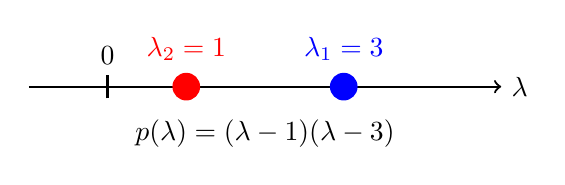
\begin{tikzpicture}
  \draw[thick, ->] (-1,0) -- (5,0) node[right] {$\lambda$};
  \draw[thick] (0,-0.15) -- (0,0.15) node[above] {$0$};
  \fill[red] (1,0) circle (5pt) node[above=6pt] {$\lambda_2=1$};
  \fill[blue] (3,0) circle (5pt) node[above=6pt] {$\lambda_1=3$};
  \node at (2,-0.6) {$p(\lambda)=(\lambda-1)(\lambda-3)$};
\end{tikzpicture}
\end{center}

%=============================================================
\section{Step-by-Step Algorithmic Workflow}
%=============================================================

\begin{learnbox}{CH Algorithm: Four Tasks}
\textbf{Task A --- Find and verify $p(A)=\mathbf{0}$}
\begin{enumerate}
  \item Write $p(\lambda) = \det(\lambda I - A)$; expand fully.
  \item Replace every $\lambda^{k}$ with $A^{k}$ and $\lambda^{0}$ with $I$.
  \item Compute $A^{2}, A^{3},\ldots$ as needed by matrix multiplication.
  \item Add all terms; confirm every entry is zero.
\end{enumerate}

\textbf{Task B --- Compute $A^{-1}$ using CH}
\begin{enumerate}
  \item Confirm $c_{0} = (-1)^{n}\det(A) \neq 0$ (matrix invertible).
  \item From $p(A)=\mathbf{0}$, factor out $A^{-1}$ after multiplying by $A^{-1}$.
  \item Express: $A^{-1} = -\tfrac{1}{c_0}(A^{n-1}+c_{n-1}A^{n-2}+\cdots+c_1 I)$.
  \item Substitute computed powers of $A$; simplify.
  \item Verify: $A \cdot A^{-1} = I$.
\end{enumerate}

\textbf{Task C --- Reduce $A^{k}$ for $k \geq n$}
\begin{enumerate}
  \item Use $A^{n} = -(c_{n-1}A^{n-1}+\cdots+c_0 I)$ as the base reduction.
  \item Iteratively compute $A^{n+1}=A\cdot A^{n}$, $A^{n+2}=A\cdot A^{n+1}$, etc.,
        substituting back after each multiplication.
  \item Express the final result as $\alpha_{k}A^{n-1}+\cdots+\beta_{k}I$.
\end{enumerate}

\textbf{Task D --- Find the minimal polynomial}
\begin{enumerate}
  \item Factorise $p(\lambda)$ into irreducible factors.
  \item For each factor $(\lambda-\lambda_i)^{m_i}$, test the smallest exponent $e_i$ ($1\leq e_i\leq m_i$)
        such that $(\lambda-\lambda_i)^{e_i}$ appears in every invariant factor of $A$.
  \item Form $m(\lambda) = \prod_{i}(\lambda-\lambda_i)^{e_i}$ and verify $m(A)=\mathbf{0}$.
\end{enumerate}
\end{learnbox}

%=============================================================
\section{Fully Worked Step-by-Step Numerical Examples}
%=============================================================

\textbf{Example 6.1 --- Verify CH for a $2\times2$ matrix}

Let $F = \begin{pmatrix} 4 & -2 \\ 1 & 1 \end{pmatrix}$.

Step 1: $p(\lambda) = \lambda^{2} - 5\lambda + 6$.

Step 2: $F^{2} = \begin{pmatrix}4&-2\\1&1\end{pmatrix}\begin{pmatrix}4&-2\\1&1\end{pmatrix}
= \begin{pmatrix}16-2&-8-2\\4+1&-2+1\end{pmatrix} = \begin{pmatrix}14&-10\\5&-1\end{pmatrix}$.

Step 3: $5F = \begin{pmatrix}20&-10\\5&5\end{pmatrix}$, $6I = \begin{pmatrix}6&0\\0&6\end{pmatrix}$.

Step 4: $p(F) = F^{2} - 5F + 6I = \begin{pmatrix}14-20+6&-10+10+0\\5-5+0&-1-5+6\end{pmatrix} = \begin{pmatrix}0&0\\0&0\end{pmatrix} = \mathbf{0}$. $\checkmark$

\bigskip

\textbf{Example 6.2 --- Find $A^{-1}$ via CH for a $3\times3$ matrix}

Let $G = \begin{pmatrix} 2 & 1 & 0 \\ 0 & 3 & 1 \\ 0 & 0 & 1 \end{pmatrix}$.

Step 1: Upper triangular, so $\det(G)=2\cdot3\cdot1=6$, $\operatorname{tr}(G)=6$.

Step 2: $G^{2}=\begin{pmatrix}4&5&1\\0&9&4\\0&0&1\end{pmatrix}$ (computed by multiplication).

Check: $G^{2}$, entry $(1,1)$: $2\cdot2+1\cdot0+0\cdot0=4$. $(1,2)$: $2\cdot1+1\cdot3=5$. $(1,3)$: $2\cdot0+1\cdot1+0\cdot1=1$. $(2,2)$: $0+9+0=9$. $(2,3)$: $0+3+1=4$. $(3,3)$: $1$. $G^{2}=\begin{pmatrix}4&5&1\\0&9&4\\0&0&1\end{pmatrix}$.

Step 3: $s_{2}=\tfrac{1}{2}(36-\operatorname{tr}G^{2})=\tfrac{1}{2}(36-14)=11$.

Step 4: $p(\lambda)=\lambda^{3}-6\lambda^{2}+11\lambda-6$. Check roots: $\lambda=1,2,3$. \checkmark

Step 5: $G^{-1}=-\tfrac{1}{-6}(G^{2}-6G+11I)=\tfrac{1}{6}(G^{2}-6G+11I)$.

$6G=\begin{pmatrix}12&6&0\\0&18&6\\0&0&6\end{pmatrix}$, $11I=\begin{pmatrix}11&0&0\\0&11&0\\0&0&11\end{pmatrix}$.

$G^{2}-6G+11I=\begin{pmatrix}4-12+11&5-6+0&1-0+0\\0-0+0&9-18+11&4-6+0\\0&0&1-6+11\end{pmatrix}=\begin{pmatrix}3&-1&1\\0&2&-2\\0&0&6\end{pmatrix}$.

$G^{-1}=\tfrac{1}{6}\begin{pmatrix}3&-1&1\\0&2&-2\\0&0&6\end{pmatrix}=\begin{pmatrix}1/2&-1/6&1/6\\0&1/3&-1/3\\0&0&1\end{pmatrix}$.

Verification: $(G)(G^{-1})$, row 1: $(2\cdot\tfrac{1}{2}+0,\; 2\cdot(-\tfrac{1}{6})+\tfrac{1}{3},\; 2\cdot\tfrac{1}{6}-\tfrac{1}{3})=(1,0,0)$. \checkmark

\bigskip

\textbf{Example 6.3 (Engineering) --- Compute $A^{8}$ for a discrete-time system state matrix}

A discrete-time linear system has state matrix $H = \begin{pmatrix} 1 & 1 \\ 0 & \frac{1}{2} \end{pmatrix}$.
The state at step $k$ is $\mathbf{x}_{k} = H^{k}\mathbf{x}_{0}$.
We wish to predict the state 8 steps ahead.

Step 1: $p(\lambda) = (\lambda-1)(\lambda-\tfrac{1}{2}) = \lambda^{2} - \tfrac{3}{2}\lambda + \tfrac{1}{2}$.
So $s = \tfrac{3}{2}$, $d = \tfrac{1}{2}$.

Step 2: By CH, $H^{2} = \tfrac{3}{2}H - \tfrac{1}{2}I$.

Verify: $H^{2}=\begin{pmatrix}1&3/2\\0&1/4\end{pmatrix}$.
$\tfrac{3}{2}H-\tfrac{1}{2}I=\begin{pmatrix}3/2&3/2\\0&3/4\end{pmatrix}-\begin{pmatrix}1/2&0\\0&1/2\end{pmatrix}=\begin{pmatrix}1&3/2\\0&1/4\end{pmatrix}$. \checkmark

Step 3: Recurrence $H^{k} = \alpha_k H + \beta_k I$ with $s=3/2$, $d=1/2$:
\[
  \alpha_{k+1} = \tfrac{3}{2}\alpha_k - \tfrac{1}{2}\alpha_{k-1},\quad
  \beta_{k+1}  = \tfrac{3}{2}\beta_k  - \tfrac{1}{2}\beta_{k-1}.
\]
Initial: $\alpha_1=1,\beta_1=0$; $\alpha_0=0,\beta_0=1$.

\begin{center}
\begin{tabular}{@{}ccc@{}}
\toprule
$k$ & $\alpha_k$ & $\beta_k$ \\
\midrule
0 & 0 & 1 \\
1 & 1 & 0 \\
2 & $3/2$ & $-1/2$ \\
3 & $3/2\cdot3/2-1/2\cdot1=7/4$ & $3/2\cdot(-1/2)-1/2\cdot0=-3/4$ \\
4 & $3/2\cdot7/4-1/2\cdot3/2=15/8$ & $3/2\cdot(-3/4)-1/2\cdot(-1/2)=-7/8$ \\
5 & $3/2\cdot15/8-1/2\cdot7/4=31/16$ & $3/2\cdot(-7/8)-1/2\cdot(-3/4)=-15/16$ \\
6 & $3/2\cdot31/16-1/2\cdot15/8=63/32$ & $3/2\cdot(-15/16)-1/2\cdot(-7/8)=-31/32$ \\
7 & $3/2\cdot63/32-1/2\cdot31/16=127/64$ & $3/2\cdot(-31/32)-1/2\cdot(-15/16)=-63/64$ \\
8 & $3/2\cdot127/64-1/2\cdot63/32=255/128$ & $3/2\cdot(-63/64)-1/2\cdot(-31/32)=-127/128$ \\
\bottomrule
\end{tabular}
\end{center}

Step 4: $H^{8} = \tfrac{255}{128}H - \tfrac{127}{128}I$.
\[
  H^{8} = \frac{255}{128}\begin{pmatrix}1&1\\0&1/2\end{pmatrix}
          - \frac{127}{128}\begin{pmatrix}1&0\\0&1\end{pmatrix}
        = \begin{pmatrix}\frac{255-127}{128} & \frac{255}{128} \\ 0 & \frac{255/2-127}{128}\end{pmatrix}
        = \begin{pmatrix}1 & \frac{255}{128} \\ 0 & \frac{1}{256}\end{pmatrix}.
\]

Step 5 (Engineering interpretation): The $(2,2)$ entry $(1/2)^{8}=1/256\approx 0.004$
shows the second state component decays to near zero after 8 steps
(stable mode), while the first component accumulates the driving effect.
The CH method avoided computing $H^{2},H^{3},\ldots,H^{8}$ independently.

%=============================================================
\section{Tabular Reference: CH Theorem vs Minimal Polynomial}
%=============================================================

\begin{center}
\renewcommand{\arraystretch}{1.4}
\begin{tabular}{@{}p{3.5cm} p{5.5cm} p{5.5cm}@{}}
\toprule
\textbf{Property} & \textbf{Characteristic Polynomial $p(\lambda)$} & \textbf{Minimal Polynomial $m(\lambda)$} \\
\midrule
Definition &
$\det(\lambda I - A)$; describes all eigenvalues with algebraic multiplicity &
Lowest-degree monic polynomial annihilating $A$ \\
Degree &
Always exactly $n$ (size of matrix) &
Between 1 and $n$; equals $n$ when $A$ has $n$ distinct eigenvalues \\
Monic &
Yes &
Yes (by definition) \\
Annihilates $A$ &
Yes (Cayley-Hamilton Theorem) &
Yes (minimal annihilating polynomial) \\
Divisibility &
$m(\lambda)$ always divides $p(\lambda)$ &
Divides any polynomial that annihilates $A$ \\
Distinct roots &
Same set as eigenvalues &
Same set as eigenvalues (but smaller multiplicities possible) \\
Equal? &
$p = m$ iff $A$ is non-derogatory (e.g., distinct eigenvalues) &
$m = p$ for most matrices encountered in engineering \\
Engineering use &
Finding eigenvalues, stability, CH-based reduction &
Determines exact reduction degree; minimal circuit depth in DSP \\
Example ($n=3$, eigenvalues $\{3,3,5\}$) &
$p(\lambda)=(\lambda-3)^{2}(\lambda-5)$ &
$m(\lambda)=(\lambda-3)(\lambda-5)$ if $A$ is diagonal \\
\bottomrule
\end{tabular}
\end{center}

%=============================================================
\section{Common Student Mistakes and Pitfalls}
%=============================================================

\begin{mistakebox}{Common Mistakes --- Cayley-Hamilton Theorem}
\begin{tabular}{@{}p{3.2cm} p{5.4cm} p{6cm}@{}}
\toprule
\textbf{Sub-Topic} & \textbf{Mistake} & \textbf{Correction} \\
\midrule
Statement \& Proof &
Claiming $p(\lambda)=0$ means the eigenvalues satisfy a scalar equation only &
$p(A)=\mathbf{0}$ is a \emph{matrix} equation; the zero on the right is the
$n\times n$ zero matrix, not the scalar 0 \\
\addlinespace
Statement \& Proof &
Confusing $\det(A-\lambda I)$ with $\det(\lambda I - A)$ and getting the wrong sign on $p$ &
Always use $p(\lambda)=\det(\lambda I - A)$; the two differ by $(-1)^{n}$,
which does not affect $p(A)=\mathbf{0}$ but can change intermediate signs \\
\addlinespace
Verification 2\(\times\)2 \& 3\(\times\)3 &
Substituting eigenvalues instead of the matrix; writing $p(\lambda_{1})=0$
and calling that ``verification of CH'' &
Verification requires forming $p(A)$ (with the matrix) and computing the result as
$\mathbf{0}$; substituting a scalar eigenvalue only confirms it is a root \\
\addlinespace
Verification 3\(\times\)3 &
Arithmetic error in $A^{3}$: computing $A^{3}$ as $(A^{2})$ then multiplying
only $n-1$ rows &
Always multiply the \emph{full} $n\times n$ matrices; check by tracing one off-diagonal entry independently \\
\addlinespace
Inverse via CH &
Dividing by $c_{0}$ when $\det(A)=0$, i.e., applying the formula to a singular matrix &
First verify $c_{0}=(-1)^{n}\det(A)\neq 0$; the formula for $A^{-1}$ is valid
only when $A$ is invertible \\
\addlinespace
Inverse via CH &
Sign error: writing $A^{-1}=\tfrac{1}{c_0}(\ldots)$ without the negative sign &
The correct formula is $A^{-1}=-\tfrac{1}{c_0}(A^{n-1}+\cdots+c_1 I)$;
the negative arises from isolating $A^{-1}$ in $p(A)=\mathbf{0}$ \\
\addlinespace
Powers via CH &
Stopping the recurrence early, e.g., writing $A^{4}=A^{2}\cdot A^{2}$ without
reducing $A^{2}$ first &
Always reduce each intermediate power to degree $< n$ before multiplying again,
or use the scalar recurrence for $\alpha_k$ and $\beta_k$ \\
\addlinespace
Powers via CH &
Assuming $A^{k}=\alpha A + \beta I$ holds for $n\times n$ matrices of any size &
The two-term form $\alpha A+\beta I$ holds only for $2\times2$; for $n\times n$,
the result is a polynomial of degree at most $n-1$ \\
\addlinespace
Minimal Polynomial &
Asserting $m(\lambda)=p(\lambda)$ for all matrices &
$m = p$ only when $A$ is non-derogatory (e.g., has $n$ distinct eigenvalues);
for diagonal matrices with repeated eigenvalues, $\deg m < \deg p$ \\
\addlinespace
Minimal Polynomial &
Forgetting that $m(\lambda)$ must be \emph{monic} &
The minimal polynomial is by definition monic; if your candidate polynomial
has a leading coefficient $\neq 1$, divide through before calling it $m(\lambda)$ \\
\bottomrule
\end{tabular}
\end{mistakebox}

%=============================================================
\section{Comprehensive Assessment Suite}
%=============================================================

\subsection*{Part A: Viva-Voce Questions}

\begin{enumerate}
  \item \textbf{(Sub-topic 1)} State the Cayley-Hamilton Theorem precisely.
        What does it mean to say ``a matrix satisfies its own characteristic equation''?
  \item \textbf{(Sub-topic 1)} In the proof sketch for a $2\times2$ matrix, at which
        step does the key cancellation occur? Why does the same argument not trivially
        extend to $n\times n$ matrices?
  \item \textbf{(Sub-topic 2)} Describe the verification procedure for a $3\times3$ matrix.
        How many matrix multiplications are required in the worst case?
  \item \textbf{(Sub-topic 2)} If you substitute a scalar eigenvalue $\lambda_1$ into $p(\lambda)$
        and get zero, have you verified the Cayley-Hamilton Theorem? Explain.
  \item \textbf{(Sub-topic 3)} Derive the formula $A^{-1} = -\tfrac{1}{c_0}(A^{n-1}+\cdots+c_1 I)$
        from $p(A) = \mathbf{0}$. What condition on $A$ is essential?
  \item \textbf{(Sub-topic 3)} For a $2\times2$ matrix with $\det(A)=0$, what happens when
        you try to apply the CH-based inverse formula?
  \item \textbf{(Sub-topic 4)} How does the relation $A^{n} = -(c_{n-1}A^{n-1}+\cdots+c_0 I)$
        guarantee that $A^{k}$ can always be expressed as a polynomial of degree $< n$ in $A$?
  \item \textbf{(Sub-topic 5)} Define the minimal polynomial. Why must it divide the characteristic
        polynomial? Give an example where they are equal and one where they differ.
  \item \textbf{(Sub-topic 5)} For a $4\times4$ matrix with characteristic polynomial
        $(\lambda-2)^{3}(\lambda-7)$, list all possible minimal polynomials.
  \item \textbf{(Sub-topics 3--4)} How does knowing the minimal polynomial speed up
        both the inverse computation and the power reduction compared to using the
        full characteristic polynomial?
\end{enumerate}

\subsection*{Part B: Descriptive Exam Questions}

\begin{enumerate}
  \item \textbf{(10 marks)} Let $A = \begin{pmatrix} 2 & 3 \\ 1 & 4 \end{pmatrix}$.
        (a) Find the characteristic polynomial $p(\lambda)$.
        (b) Verify the Cayley-Hamilton Theorem by computing $p(A)$ directly.
        (c) Use the CH relation to find $A^{-1}$.
        (d) Hence compute $A^{4}$.
        \emph{Hint: first reduce $A^{2}$ via CH, then build up $A^{3}$ and $A^{4}$.}

  \item \textbf{(10 marks)} For the matrix $B = \begin{pmatrix}0 & 1 & 0\\0 & 0 & 1\\1 & -3 & 3\end{pmatrix}$:
        (a) Compute the characteristic polynomial.
        (b) Verify the Cayley-Hamilton Theorem.
        (c) Using CH, find $B^{-1}$.
        \emph{Hint: $B$ is a companion matrix; its characteristic polynomial factors nicely.}

  \item \textbf{(8 marks)} A state-space system has matrix $K = \begin{pmatrix} 0 & 1 \\ -2 & 3 \end{pmatrix}$.
        Using the Cayley-Hamilton Theorem, compute $K^{6}$ as a linear combination of $K$ and $I$.
        Then evaluate $K^{6}$ numerically.
        \emph{Hint: Set up the scalar recurrence for $\alpha_k$ and $\beta_k$ using
        $s=\operatorname{tr}K$ and $d=\det K$.}

  \item \textbf{(6 marks)} Let $M = \operatorname{diag}(2, 2, 5)$.
        (a) Write down $p(\lambda)$.
        (b) Show that $m(\lambda) = (\lambda-2)(\lambda-5)$ annihilates $M$.
        (c) Explain why $m \neq p$ and what property of $M$ causes this.

  \item \textbf{(8 marks)} Given $A = \begin{pmatrix} 3 & -1 \\ 1 & 1 \end{pmatrix}$,
        compute $f(A)$ where $f(\lambda) = \lambda^{7} - 4\lambda^{6} + 3\lambda^{5}$
        using the Cayley-Hamilton Theorem.
        Express the answer as a polynomial of degree $\leq 1$ in $A$.
        \emph{Hint: First find $p(\lambda)$, then perform polynomial long division
        $f(\lambda) \div p(\lambda)$ to find the remainder $r(\lambda)$.}
\end{enumerate}

\subsection*{Part C: Multiple Choice Questions}

\begin{enumerate}
  \item \textbf{(Sub-topic 1)} The Cayley-Hamilton Theorem states that for an $n\times n$ matrix $A$
        with characteristic polynomial $p(\lambda)$:
        \begin{enumerate}[label=\Alph*.]
          \item $p(\lambda) = 0$ has $n$ real roots
          \item \textbf{$p(A) = \mathbf{0}$ (the $n\times n$ zero matrix)}
          \item $A p(\lambda) = 0$ for all scalars $\lambda$
          \item $p(A) = I$
        \end{enumerate}
        \emph{Explanation: The theorem asserts that substituting the matrix $A$ for $\lambda$ in the
        characteristic polynomial yields the zero matrix, not a scalar zero.}

  \item \textbf{(Sub-topic 2)} For $A = \begin{pmatrix}1&2\\3&4\end{pmatrix}$, the characteristic
        polynomial is $p(\lambda)=\lambda^{2}-5\lambda-2$. When we verify CH, we compute:
        \begin{enumerate}[label=\Alph*.]
          \item $p(1) = 0$ and $p(4) = 0$
          \item \textbf{$A^{2} - 5A - 2I = \mathbf{0}$}
          \item $A^{2} = 5A$
          \item $(A-I)(A-4I) = \mathbf{0}$
        \end{enumerate}
        \emph{Explanation: Verification substitutes $A$ (the matrix) into the characteristic polynomial,
        not its eigenvalue roots.}

  \item \textbf{(Sub-topic 3)} If $p(\lambda)=\lambda^{2}-5\lambda+6$ is the characteristic
        polynomial of invertible $A$, then $A^{-1}$ equals:
        \begin{enumerate}[label=\Alph*.]
          \item $\tfrac{1}{6}(A+5I)$
          \item $\tfrac{1}{5}(A-6I)$
          \item \textbf{$\tfrac{1}{6}(A-5I)$}  \quad [i.e., $-\tfrac{1}{6}(A^{1} + (-5)I) = \tfrac{1}{6}(5I-A)$, equivalently $\tfrac{1}{6}(5I-A)$]
          \item $6(A-5I)$
        \end{enumerate}
        \emph{Explanation: From $A^{2}-5A+6I=\mathbf{0}$, multiply by $A^{-1}$:
        $A - 5I + 6A^{-1}=\mathbf{0}$, so $A^{-1}=\tfrac{1}{6}(5I-A)$.}

  \item \textbf{(Sub-topic 4)} For a $2\times2$ matrix $A$ with $p(\lambda)=\lambda^{2}-3\lambda+2$,
        the expression $A^{3}$ using CH equals:
        \begin{enumerate}[label=\Alph*.]
          \item $9A - 6I$
          \item $6A - 4I$
          \item \textbf{$7A - 6I$}
          \item $3A - 2I$
        \end{enumerate}
        \emph{Explanation: $A^{2}=3A-2I$. $A^{3}=A(3A-2I)=3A^{2}-2A=3(3A-2I)-2A=7A-6I$.}

  \item \textbf{(Sub-topic 5)} For a diagonal matrix $A = \operatorname{diag}(4,4,9)$, the minimal
        polynomial is:
        \begin{enumerate}[label=\Alph*.]
          \item $(\lambda-4)^{2}(\lambda-9)$
          \item $(\lambda-4)(\lambda-9)^{2}$
          \item \textbf{$(\lambda-4)(\lambda-9)$}
          \item $(\lambda-4)^{2}(\lambda-9)^{2}$
        \end{enumerate}
        \emph{Explanation: For a diagonal matrix, the minimal polynomial has each distinct eigenvalue
        appearing with exponent 1, regardless of algebraic multiplicity in $p(\lambda)$.}

  \item \textbf{(Sub-topics 1, 5)} Which of the following is always true?
        \begin{enumerate}[label=\Alph*.]
          \item The minimal polynomial equals the characteristic polynomial
          \item \textbf{The minimal polynomial divides the characteristic polynomial}
          \item The characteristic polynomial divides the minimal polynomial
          \item The minimal and characteristic polynomials share no common roots
        \end{enumerate}
        \emph{Explanation: By the Cayley-Hamilton Theorem and the definition of minimal polynomial,
        $m(\lambda)$ always divides $p(\lambda)$.}
\end{enumerate}

%=============================================================
\section{Quick Recap and Formula Sheet}
%=============================================================

\begin{learnbox}{Cayley-Hamilton Theorem --- Key Formulas and Facts}
\begin{itemize}
  \item \textbf{CH Theorem:} Every $n\times n$ matrix $A$ satisfies its own characteristic equation:
        $p(A) = A^{n} + c_{n-1}A^{n-1} + \cdots + c_{1}A + c_{0}I = \mathbf{0}$.
  \item \textbf{Inverse via CH (invertible $A$ only):}
        $A^{-1} = -\dfrac{1}{c_{0}}\!\left(A^{n-1} + c_{n-1}A^{n-2} + \cdots + c_{1}I\right)$,
        where $c_{0} = (-1)^{n}\det(A) \neq 0$.
  \item \textbf{$2\times2$ shortcut:}
        $A^{-1} = \dfrac{1}{\det(A)}\!\left(\operatorname{tr}(A)\,I - A\right)$.
  \item \textbf{Power reduction:} Express $A^{n}$ from CH and iterate:
        $A^{n} = -(c_{n-1}A^{n-1}+\cdots+c_{0}I)$;
        any $A^{k}$ ($k\geq n$) reduces to $\alpha_{n-1}A^{n-1}+\cdots+\alpha_{0}I$.
  \item \textbf{Minimal polynomial $m(\lambda)$:} Lowest-degree monic polynomial with $m(A)=\mathbf{0}$;
        $m(\lambda)$ divides $p(\lambda)$ and has the same \emph{distinct} roots.
  \item \textbf{When $m=p$:} $A$ has $n$ distinct eigenvalues, or is a companion matrix.
        When $m \subsetneq p$: $A$ is diagonal (or block-diagonal) with repeated eigenvalues.
  \item \textbf{Engineering payoff:} CH converts $A^{k}$ (any $k$) into $O(n^{3})$ operations
        instead of $O(kn^{3})$ brute-force multiplications---critical for real-time control and
        long-horizon simulation.
  \item \textbf{Quick verification checklist:}
        (1) Compute $p(\lambda)$. (2) Form $p(A)$. (3) Check all entries are zero. (4) Done.
\end{itemize}
\end{learnbox}

\end{document}
